\section{Application Scenarios}
\label{sec:caseStudy}
% \shusen{A full case study that driven by the visualization task and the question associated with them}
%In this section, we discuss application scenarios, in which the domain experts utilize the
To better illustrate how the proposed perturbation-driven exploration tool helps researchers interpret the neural network model, we present five application scenarios gathered by the domain experts who integrated the proposed tool in their analysis workflow.

\subsection{Scenario 1: Assess the Model Prediction Stability}
The robustness of the prediction is often hard to evaluate. However, the prediction stability provides valuable information for the researchers to better understand the model.
%
In the proposed work, we approach the prediction robustness from sensitivity analysis point of view. The stability of the prediction is measured by how often the predicted labels are altered after small perturbations are applied to the input.
%
Compare to other types of input (e.g., image), perturbation of the natural language can be particularly tricky, as small alteration of words can drastically change the meaning of the sentence. As discussed in Section~\ref{sec:sentence}, we try to maintain semantic of the sentence by only replace words with their synonymous and only replace one word for each pair.
As illustrated in Fig.~\ref{fig:predictStability}, by utilizing the proposed tool, the domain expert can not only examine a visual summary of the stability but also quickly dive into individual examples for case by case analysis.

\begin{figure}[htbp]
\centering
\vspace{-2mm}
 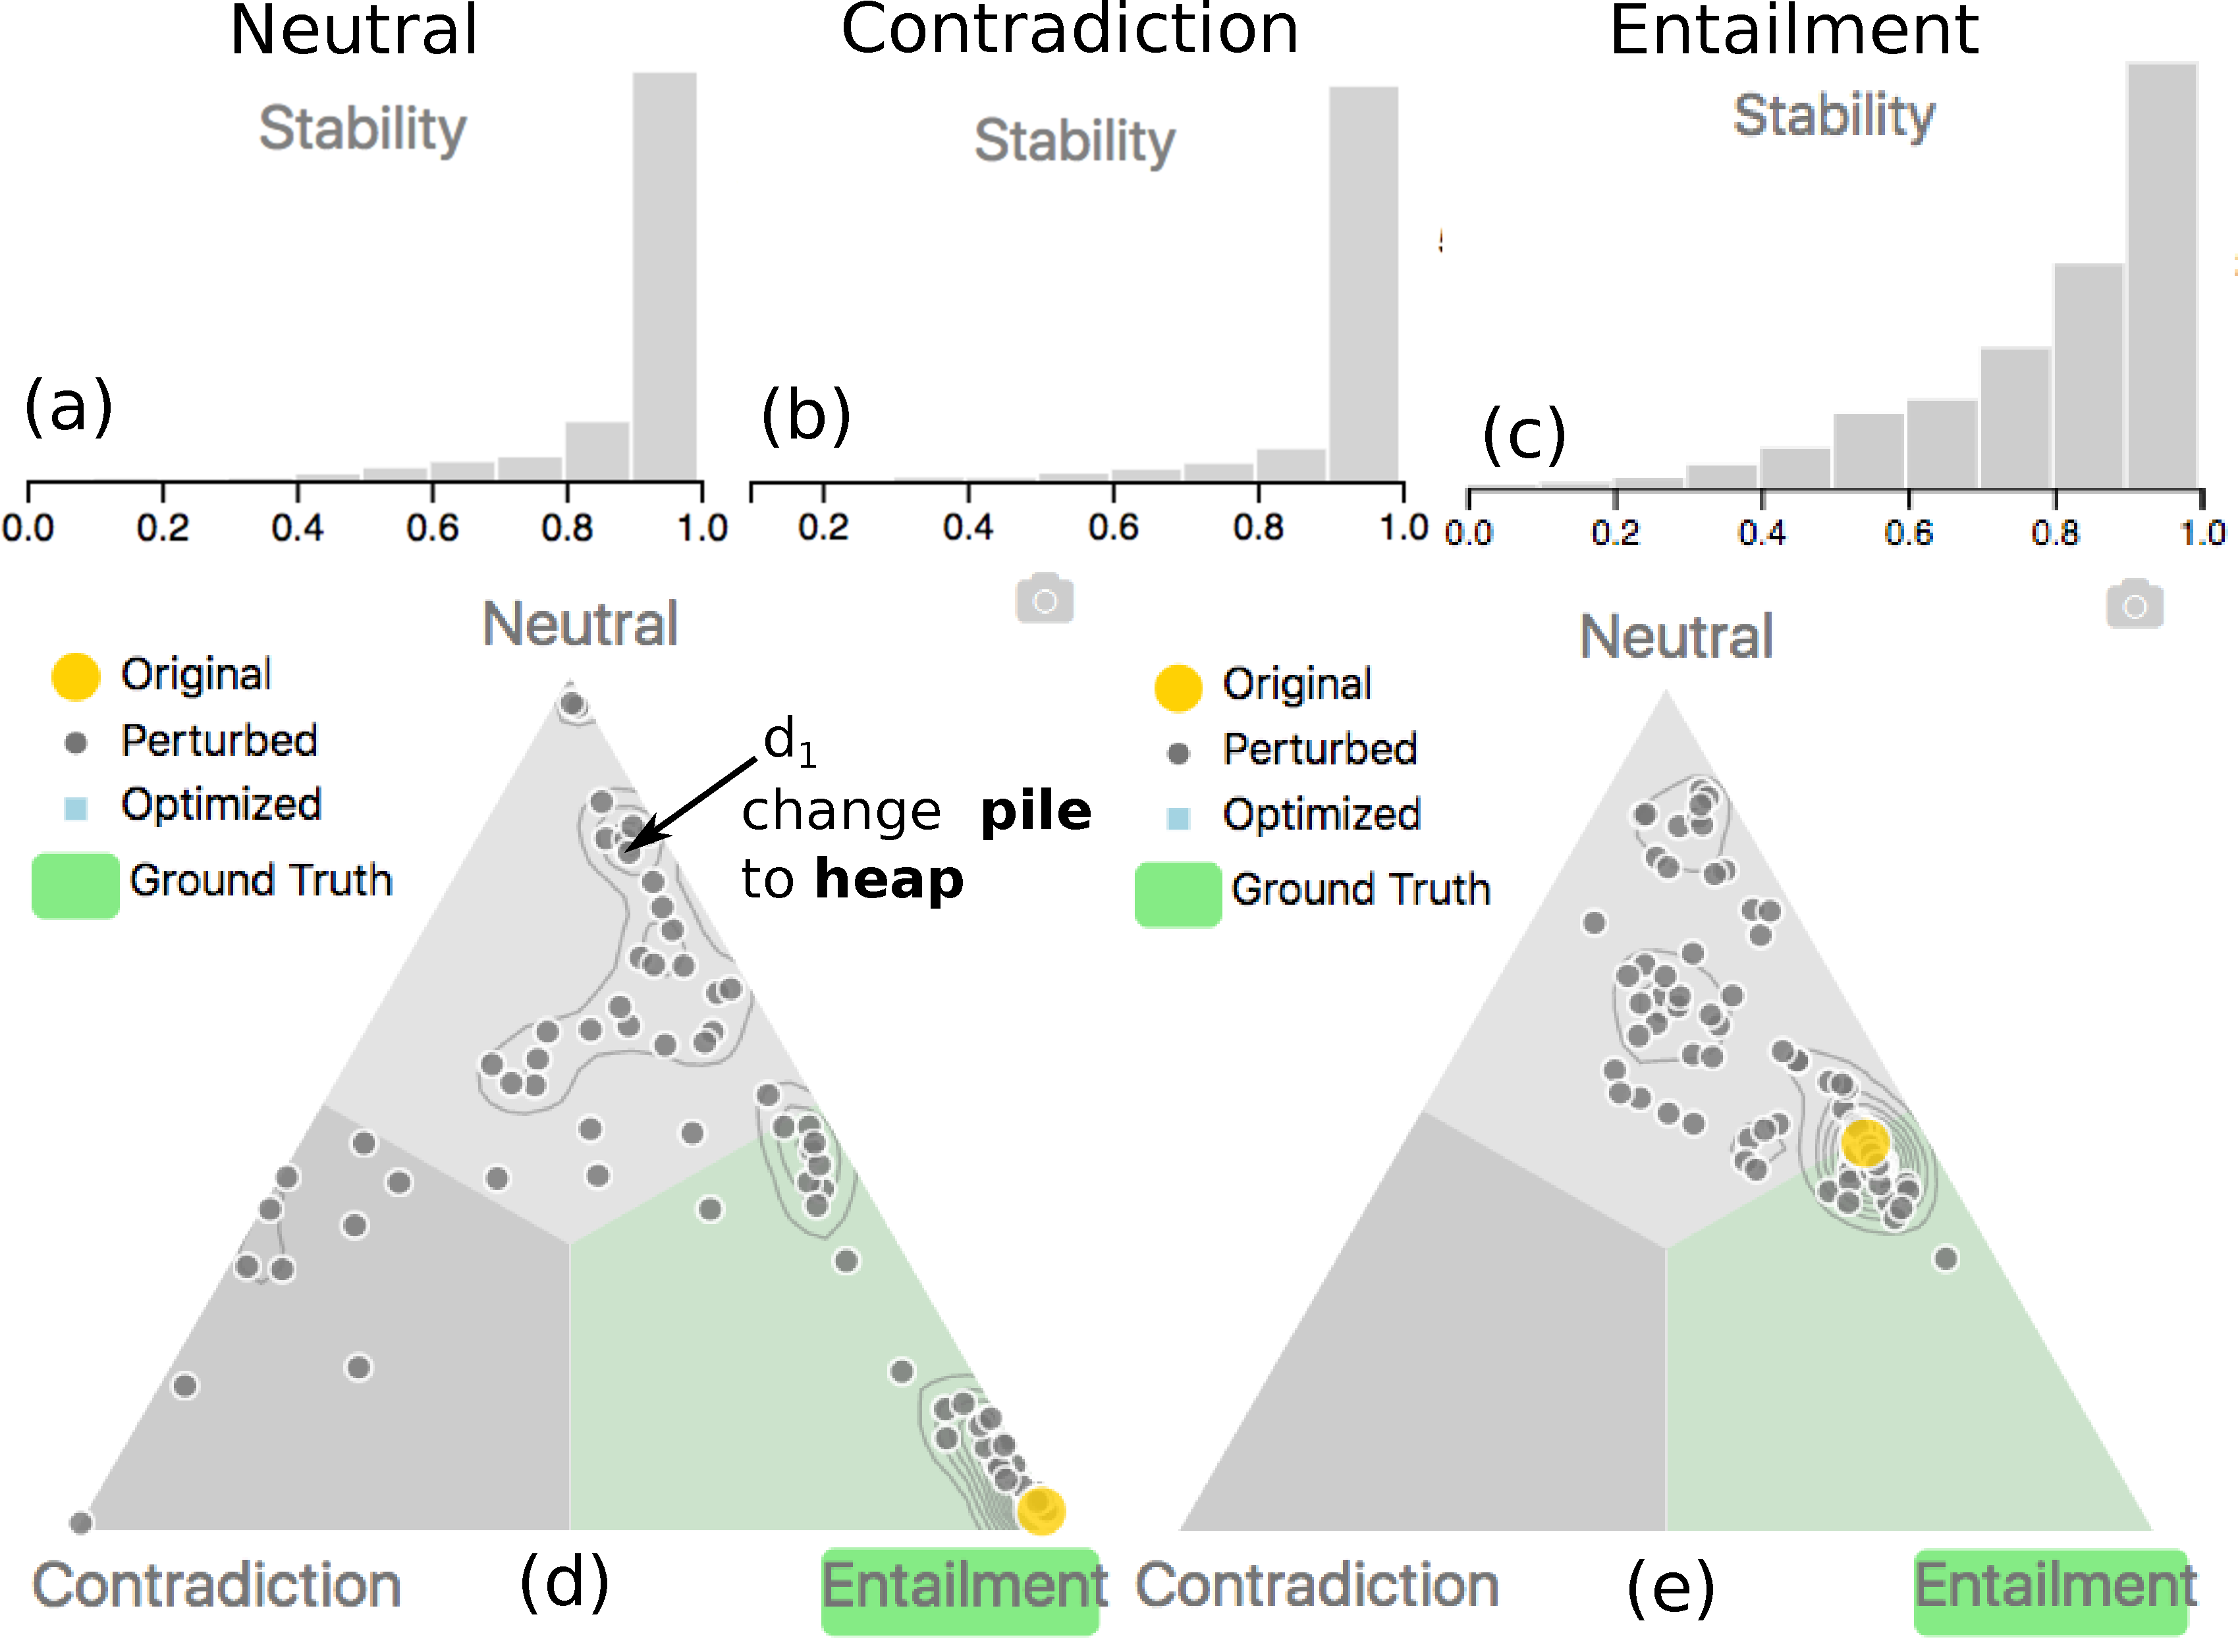
\includegraphics[width=1.0\linewidth]{predictStability}
 \vspace{-4mm}
 \caption{
Prediction stability assessment. In (a)(b)(c), we estimate the overall prediction stability (regarding synonymous perturbation) for each type prediction over the entire development set (10k examples). The user can drill down to individual examples by filtering via the histogram or scatterplot (see Fig.~\ref{fig:summaryView}). For highly unstable prediction, we often observe the original prediction is near a decision boundary (e.g., the yellow circle in (e) corresponds to a prediction that is at the boundary between \emph{entailment} and \emph{neutral}), however, some predictions, such as the one illustrated in (d) can alter the prediction quite drastically with minor perturbation (illustrated in $d_1$, where the word \textbf{pile} is replaced by \textbf{heap} in the hypothesis sentence).
}
\label{fig:predictStability}
\vspace{-2mm}
\end{figure}

In Fig.~\ref{fig:predictStability}(a)(b)(c), we compare the overall prediction stability (regarding synonymous perturbation) for all correct predictions in the development set (10k examples in total).
%
We observe a drastic difference for the stability for \emph{entailment} predictions compare to the \emph{contradiction} and \emph{neutral} ones.
%
Such a distinction can be partially explained by how \emph{entailment} relationship is defined. The relationship is only valid if the concept in the premise is more specific than the concept in the hypothesis. Therefore, the synonymous perturbation may change the \emph{entailment} relationship, as the replaced \emph{noun} or \emph{verb} can be more or less restrictive compared to the original.
This inherent disparity of sensitivity may worth extra consideration when designing future NLI models.

Besides presenting the summary view, the tool also allows the user to quickly narrow down the selection to a single example by filtering via the histogram and scatterplot (see Fig.~\ref{fig:summaryView}).
%
Through the exploration of many samples with low stabilities (i.e., high sensitivities values in the plots), domain experts notice that many highly unstable outliers are from sentence pairs where the predictions are near the decision boundary (see Fig.~\ref{fig:predictStability}(e), the yellow circle corresponds to a \emph{entailment} prediction that is very close to \emph{neutral}).
However, some predictions, such as the one illustrated in Fig.~\ref{fig:predictStability}(d) can alter the prediction quite drastically with minor perturbation (shown in Fig.~\ref{fig:predictStability}$d_1$, where the word \textbf{heap} is replaced by \textbf{pile} in the hypothesis sentence). In the following section, we will examine what happened inside the model and hypothesize the cause of failure (see Fig.~\ref{fig:att2pred}).

%%%%%%%%%%%%%%%%%%%%%%%%%%%%%%%%%%%%%%%%%%%%%%%
% perturb input, attention
\subsection{Scenario 2: Examine the Decision Making Process}
The predicted label alone provides limited information. Often, domain experts want to know how does the model arrive at a conclusion. And if the prediction is incorrect, where in the model does the error occur?
Examining the decision making process is not only instrumental in evaluating the model performance but also essential for hypothesizing improvement strategies for future models.
%
In the NLI model, the three stages (encoder, attention, classifier) work in synergy to produce the prediction.
Therefore, making sense of the prediction involves understanding how different parts of the model affect the final prediction.

In the previous section, we have noticed that a minor perturbation of the sentence may result in change of the final prediction (Fig.~\ref{fig:predictStability}(d)). Here, we want to make sense of what lead to the failed prediction. In this example, the premise \textbf{P} is ``A very young child in a red plaid coat and pink winter hat makes a snowball in a large \textbf{pile} of snow.'', and the original hypothesis \textbf{H1} is ``A child in a red plaid coat and pink winter hat makes a snowball in a large \textbf{pile} of snow.''. The perturbed hypothesis \textbf{H2} replaces the word \textbf{pile} with \textbf{heap} in \textbf{H1}. This example should be rather straightforward for the model since there are only minor differences between the \textbf{P} and \textbf{H1}/\textbf{H2}.

\begin{figure}[htbp]
\centering
\vspace{-2mm}
 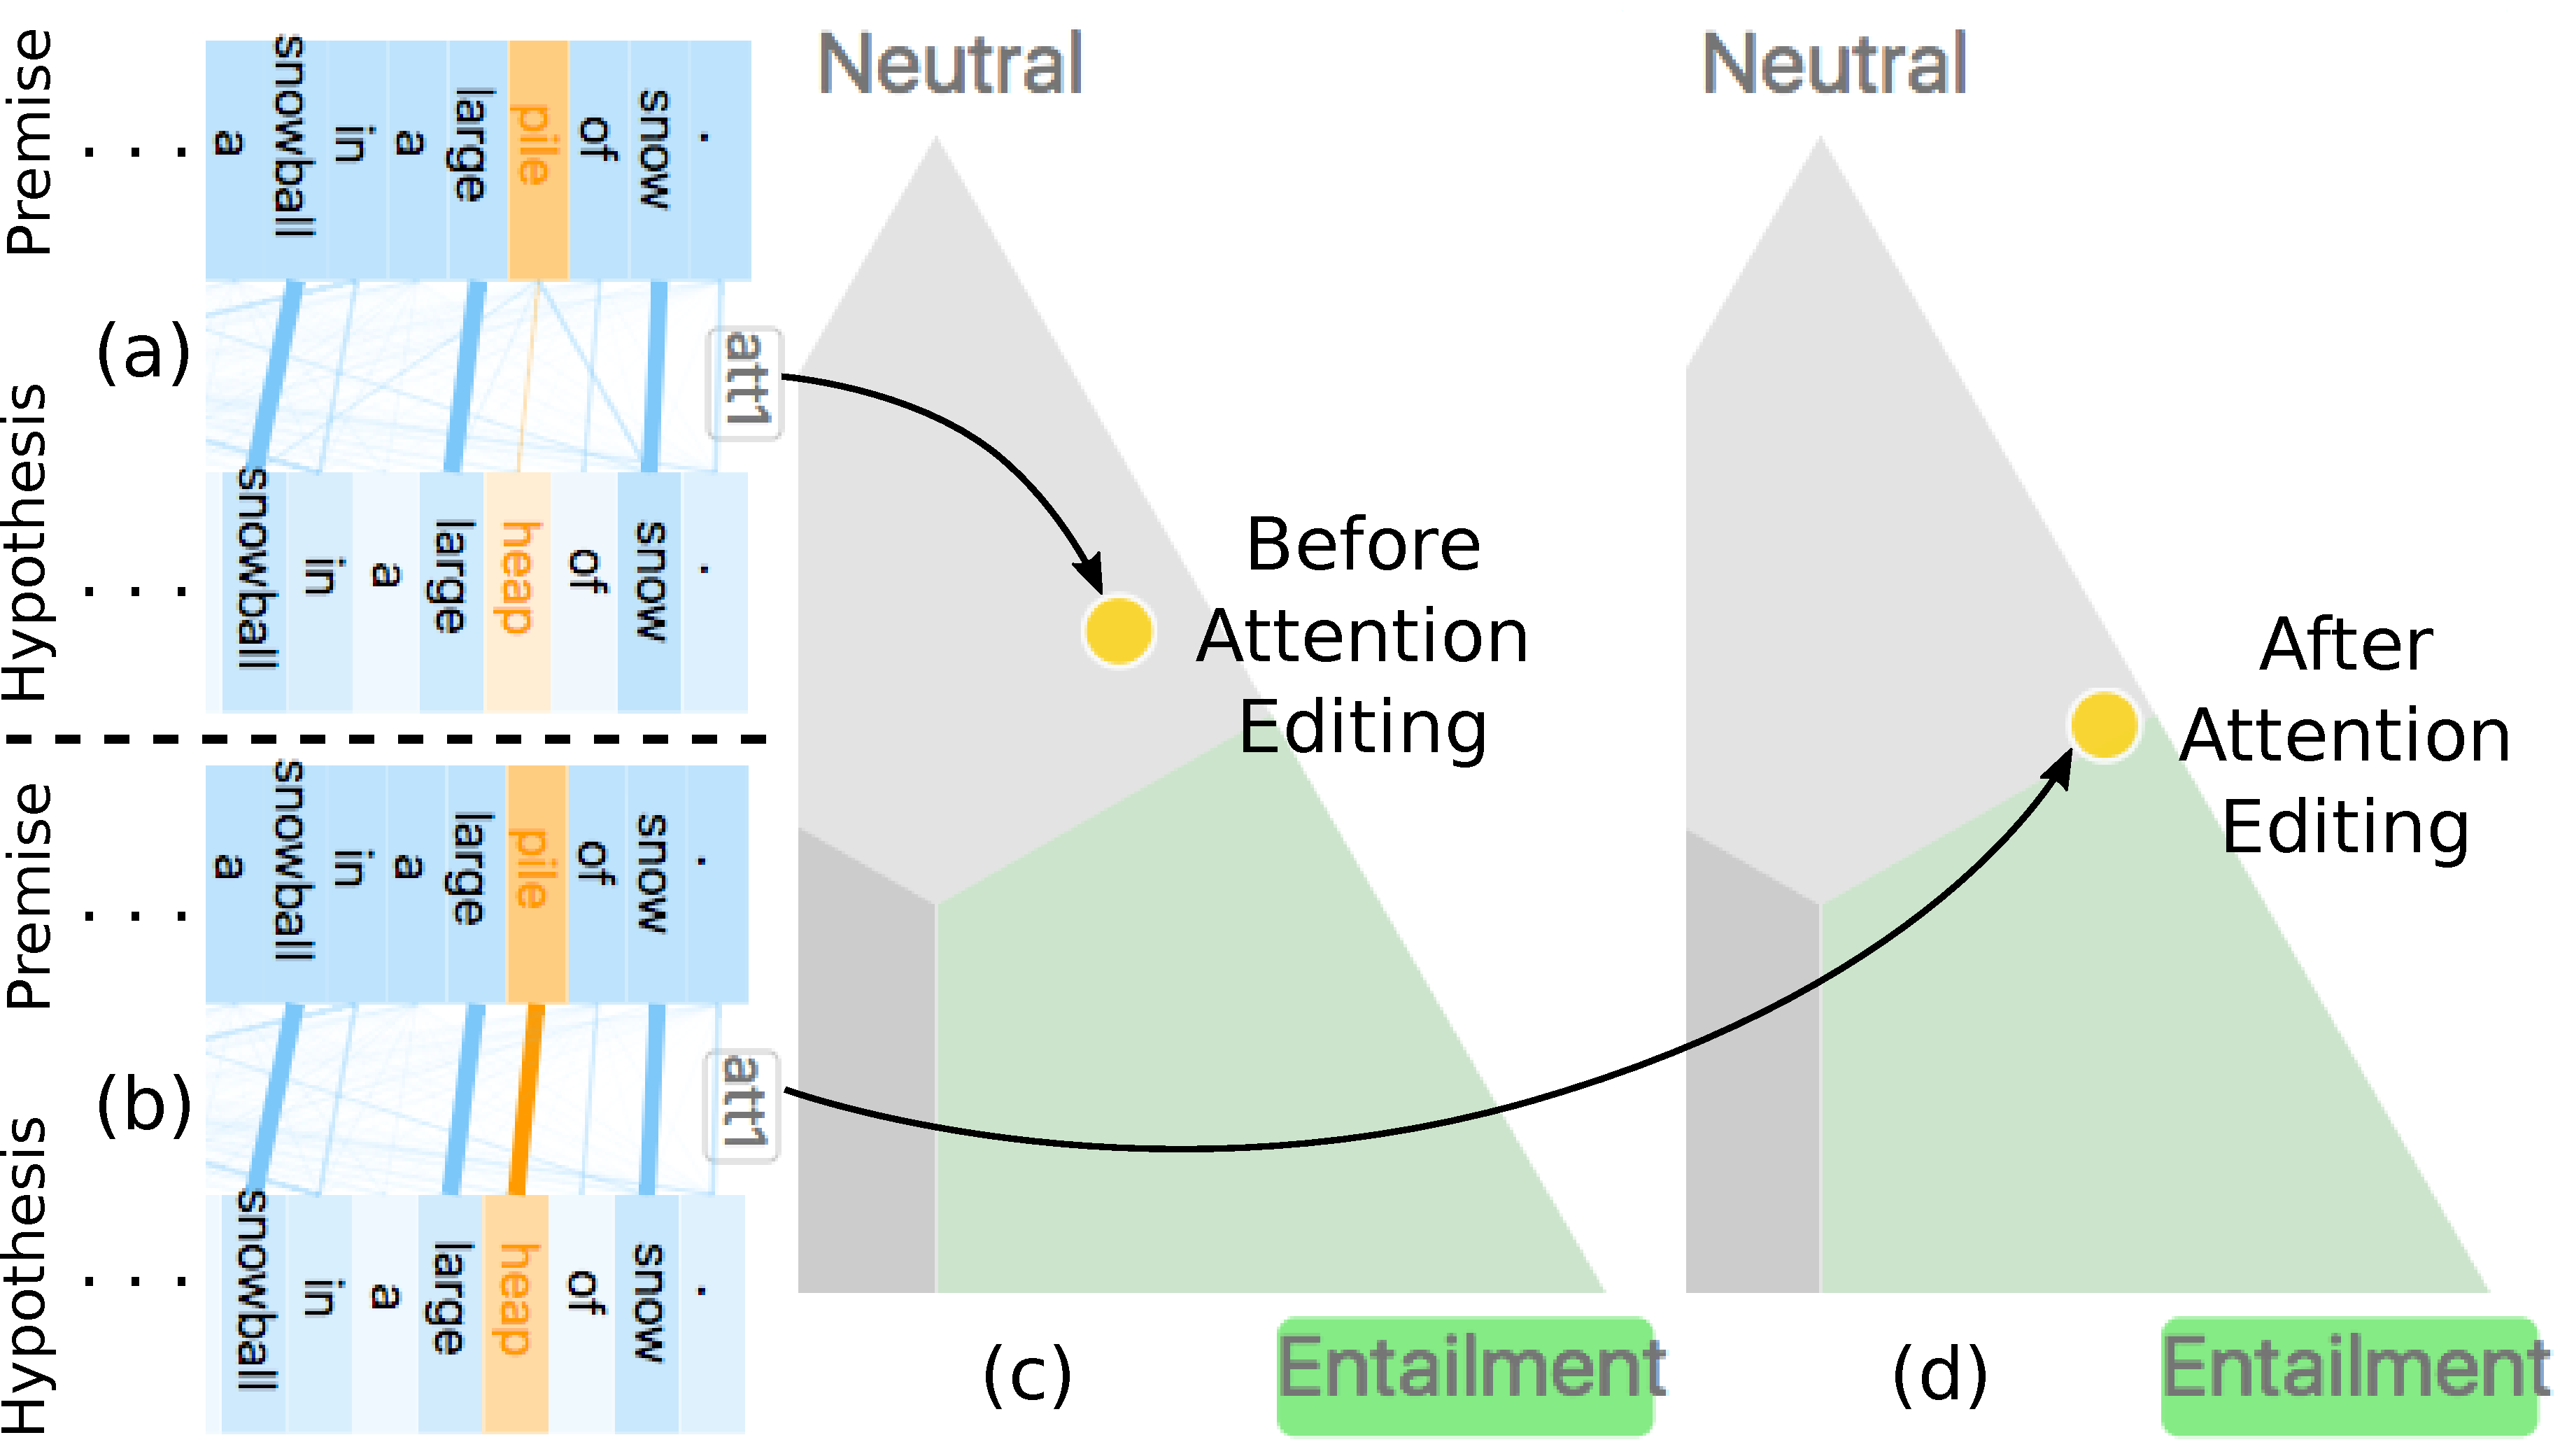
\includegraphics[width=1.0\linewidth]{att2pred}
 \caption{
Editing the original attention (a) to correctly align the word "heap" with "pile" as shown in (b) (these two words are highlighted in orange).
The change of attention leads to the change of prediction from neutral to the class boundary between \emph{neutral} and \emph{entitlement}.
%
}
\label{fig:att2pred}
\end{figure}

As illustrated in Fig.~\ref{fig:att2pred}(a), based on the graph attention visualization, we can see in the attention for (\textbf{P}, \textbf{H2}) pair, the word \textbf{pile} and \textbf{heap} is not well-aligned (see Fig.~\ref{fig:att2pred}(a)).
%
To test whether the alignment is what contribute to the misclassification, the domain expert utilizes the attention editing functionality in the matrix attention view (Fig.~\ref{fig:attentionVis}(c)) to make the word \textbf{pile} align with \textbf{heap} (shown in Fig.~\ref{fig:att2pred}(b)).
%
As illustrated in Fig.~\ref{fig:att2pred} (d), after the edit, the original prediction (Fig.~\ref{fig:att2pred}(c)) has been moved from neutral to the classification boundary (Fig.~\ref{fig:att2pred}(d)), but the corrected attention fails to produce a conclusive \emph{entailment} prediction (a case where the attention edit corrects the final prediction is shown in Fig.~ref{fig:depTreeExample}).
%
%Interestingly, the original pair's attention is almost identical to the edited attention (the comparison is not shown in the figure). 
Such an observation implies that the model does not firmly believe ``\textbf{heap} of snow'' and ``\textbf{pile} of snow'' have the same meaning, which may indicate the potential issue with the encoder or word embedding.


%\begin{figure}[htbp]
%\centering
%\vspace{-2mm}
% 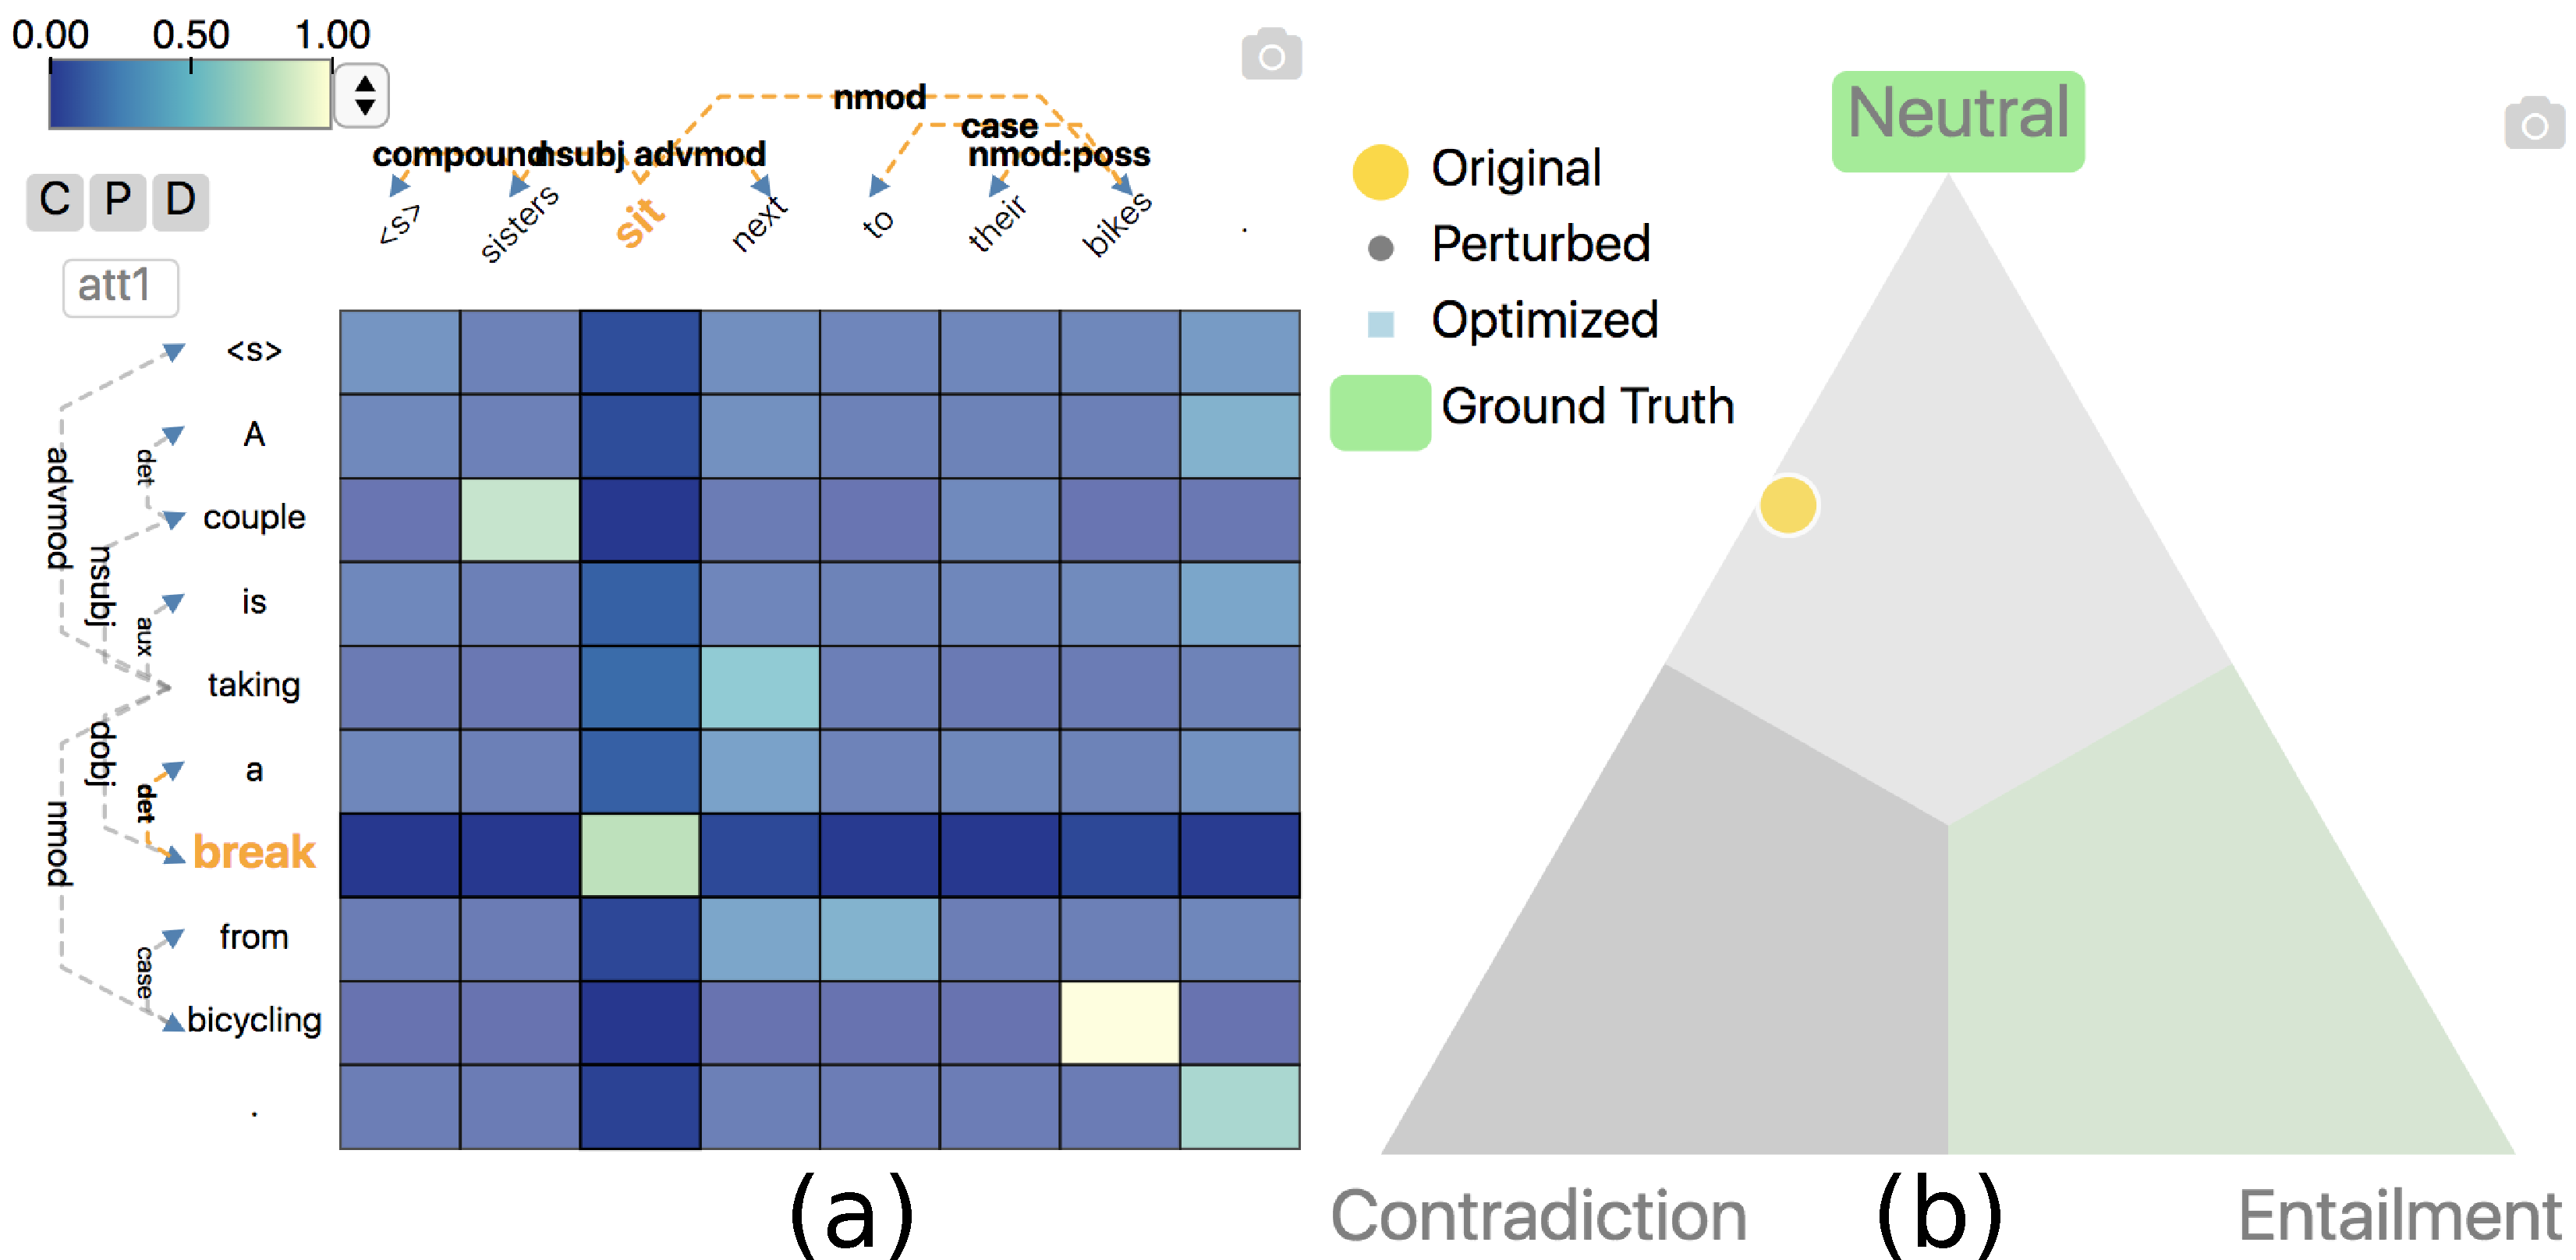
\includegraphics[width=1.0\linewidth]{wrongAlignRightPred}
% \caption{
%The model may produces the right prediction for the ``wrong'' reason, i.e., attention.
%The word \textbf{break} and \textbf{sit} should not align with each other (a). Yet, based on the attention, model still produces the correct prediction (b).
%}
%\label{fig:wrongAlignRightPred}
%\end{figure}


%\shusen{Example where the prediction is correct but the alignment is wrong}
%%%% are we obtain correct prediction from wrong alignment %%%%%
%By looking into the model decision making process, we can assess whether the model is behaving as intended. For the attention based NLI model, one underlying assumption is that the attention should capture the correct alignment between words in the premise and hypothesis sentence for the classifier to make an informed/correct decision.
We have shown that the perfect alignment does not necessarily guarantee a correct prediction.
%
On the flip side, we may produce the right predictions for the ``wrong'' reason (i.e., incorrect attention). 
%As illustrated in Fig.~\ref{fig:wrongAlignRightPred}, 
For example, in the sentence pair (\textbf{P}: ``A couple is taking a break from bicycling.'', \textbf{H}: ``sisters sit next to their bikes.''), the word \textbf{take} and \textbf{next} should not align with each other,
%(Fig.~\ref{fig:wrongAlignRightPred}(a)), 
yet, it still produce the correct \emph{neutral} label.% (Fig.~\ref{fig:wrongAlignRightPred}(b)).

%By looking into the model decision making process, we can assess whether the model is behaving as intended. 
%These situations demonstrate the important of understanding the model decision making process, we can assess whether the model is behaving as intended. 


%%%% hypothesis on which part of model is wrong? %%%%%


%One of the essential task for can be made in either of these stages.
% \shusen{difference in sensitivity among entail natural and contradict relationships}
% the generate the correct prediction for the wrong reason


%%%%%%%%%%%%%%%%%%%%%%%%%%%%%%%%%%%%%%%%%%%%%%%
\subsection{Scenario 3: What Does It Take to Correct a Failed Prediction?}
Up till now, we have employed perturbation for input to understand prediction robustness, utilized the perturbation of attention (and input) to infer the model decision making process. Both these perturbation operations rely on forward propagation in the pipeline and assume the model parameter stay unchanged.
%
However, once we get a sense of how predictions are made and hypothesized about the cause of failure in case of a prediction error, it is natural to ask the follow-up questions. What does it take to fix an incorrect prediction? And more importantly, what role does each of the three stages play in such a process? Are they affecting the prediction differently?

Domain experts can obtain answers to these questions by utilizing the prediction and pipeline view in the proposed. As discussed in details in Section~\ref{sec:pipeline}, we employed an margin-infused relaxed algorithm (MIRA) based optimization with two objectives (1. apply least amount of change to the parameter, 2. make the new prediction as close to the reassigned prediction as possible) to update the network parameters.
%
We then visualize how much each stage of the model is changed through the distribution of parameters difference (see Fig.~\ref{fig:pipelineView}).

\begin{figure*}[t]
\centering
\vspace{-2mm}
 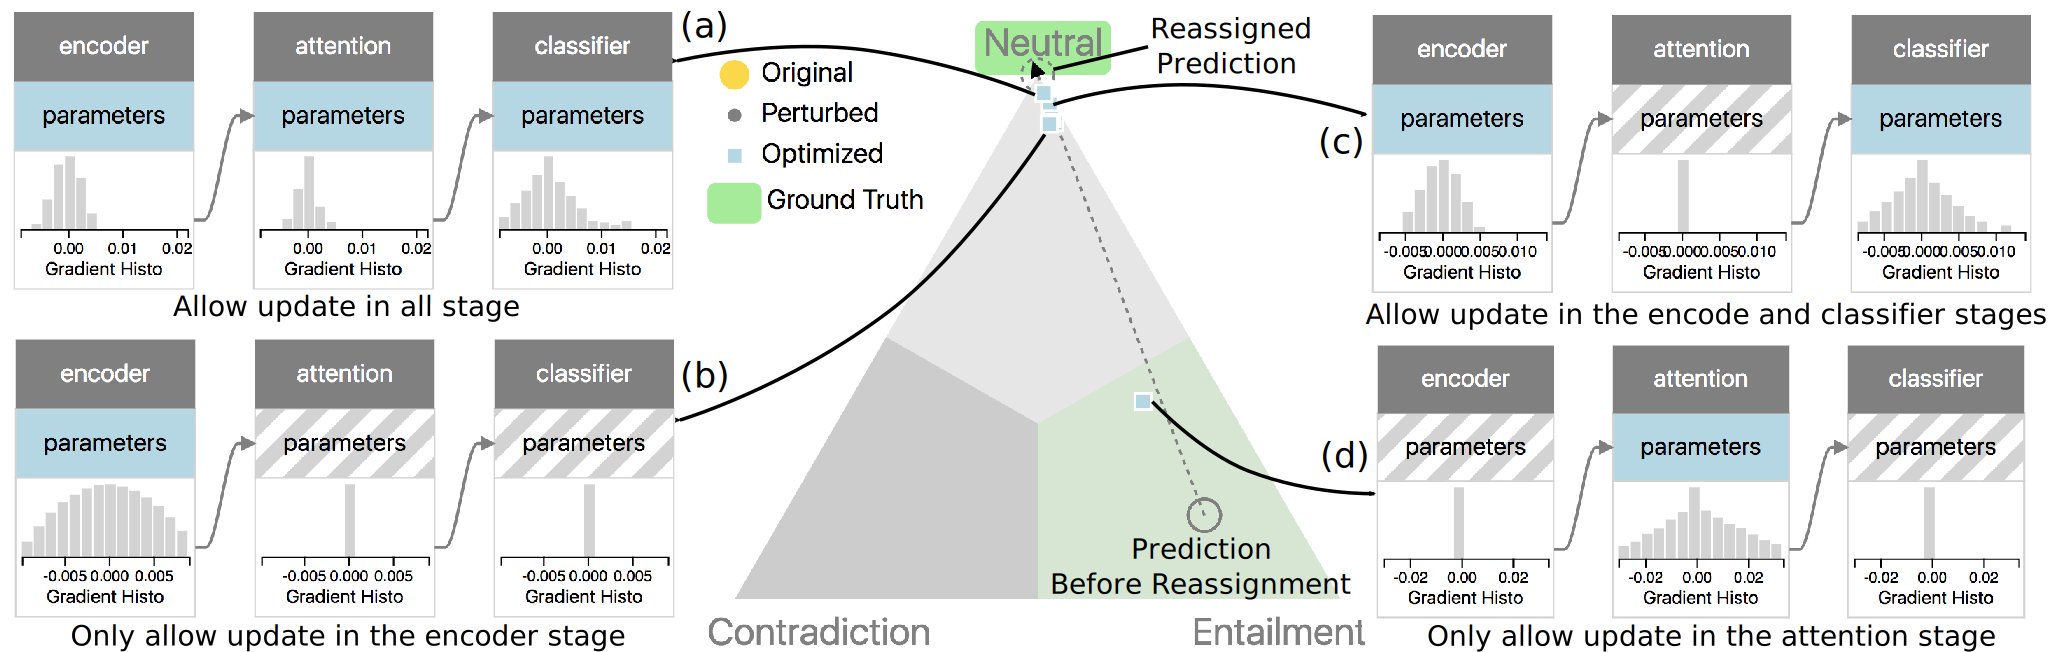
\includegraphics[width=1.0\linewidth]{pipelineUpdate}
  \vspace{-6mm}
 \caption{
Experiment with all configurations for the label reassignment optimization. As shown in (d), the update of attention stage seems to have significantly less impact on the prediction result compared to the classifier or encoder of the model.
 }
\label{fig:pipelineUpdate}
\end{figure*}

To infer the role each stage of the pipeline plays, the proposed tool allows the parameter update to be enabled or disabled for each pipeline stage.
The tool also includes an automatic option to test all the possible configuration combinations. As illustrated in Fig.~\ref{fig:pipelineUpdate}, the ground truth for this sentence pair is neutral. However, the model produces an incorrect label \emph{entailment}. The domain expert reassigns the prediction to \emph{neutral}, which triggers the prediction update optimization for $7$ different pipeline configurations. Four configurations are shown in Fig.~\ref{fig:pipelineUpdate}(a)(b)(c)(d). The updated predictions are illustrated as blue squares, and the pointers highlighted the corresponding pipeline configurations.

Interestingly, all configurations except one are concentrated around the full \emph{neutral} prediction. Referring back to the pipeline visualization, we observe that the only configuration that failed to produce the correct label is the one, in which we only allow to update attention stage of the model.
%
In other words, the update of attention stage seems to have significantly less impact on the prediction result compared to the classifier or encoder of the model. Similar observation can be obtained for most examples we experimented.
%The attention layer is less sensitive compared to encoding layer and classification layer.
%When examined other sentences pairs, such an observation remains.
%This gives domain expert some hint about the significance of the role of each pipeline stage play in this model.
% which based on the natural extension of the margin-infused relaxed algorithm (MIRA) to the neural network generalize the concept of maligin combined effort of the  proposed technique

%
%However, to understand how the model should
\begin{figure*}[t]
\centering
\vspace{-2mm}
 \includegraphics[width=1.0\linewidth]{depTreeExample}
  \vspace{-6mm}
 \caption{
Dependency tree provides valuable information that can help fix the prediction error.
In (a), the model mistakenly aligns the word green, which lead to wrong prediction.  
After examining the dependency tree (highlighted by pink squares), we can see the two \textbf{green} are attached to different words.
In (b), by editing the attention and forcing the two \textbf{green}'s alignment to be zero, the prediction label is corrected to \emph{neutral}. 
 }
\label{fig:depTreeExample}
 \vspace{-2mm}
\end{figure*}

%%%%%%%%%%%%%%%%%%%%%%%%%%%%%%%%%%%%%%%%%%%%%%%
\subsection{Scenario 4: Explore Relationship Between Grammar and Attention}
The attention computation in the NLI model does not take the grammar structure of the sentences into consideration,
yet, the attention often highlight key elements of the sentence. 
Therefore, domain experts wish to understand whether attention alone is sufficient to capture sentence structure. 
And more important what kind of benefit can the additional information from grammar parsing help address the NLI challenge.

In the proposed system, we overlay the sentence dependency tree with the attention, which enables researchers to conduct comparisons between attention and grammar structure.
As illustrated in Fig.~\ref{fig:depTreeExample}(a), the prediction of the sentence pair (\textbf{P}:``A woman in a green jacket is drinking tea.'' \textbf{H}:``A woman is drinking green tea.'') is wrong. We can infer the cause by examining the attention, in which the word \textbf{green} in ``\textbf{green} jacket" is aligned to the \textbf{green} in ``\textbf{green} tea". Due to such an alignment, the model mistakenly believe the two \textbf{green} are used to describe the same thing (therefore, predict \emph{entailment}).  However, as we examine the dependency tree, the two \textbf{green} are attached to different words, i.e., ``green" in \textbf{P} is attached to jacket, while ``green" in \textbf{H} to tea. Therefore, they should not be aligned to allow the classifier make the right decision.
%
This experiment demonstrates the potential benefit to include grammar structure in the alignment computation. %This stresses the importance of dependency tree in our tool.
%
And interestingly, as illustrated in Fig.~\ref{fig:depTreeExample}(b), by editing the attention and forcing the two \textbf{green}'s alignment to be zero, the prediction label is corrected (\emph{neutral}). 

%%%%%%%%%%%%%%%%%%%%%%%%%%%%%%%%%%%%%%%%%%%%%%%
\subsection{Scenario 5: Handcraft Example Exploration}
To test the limits of the model, domain experts often handcraft ``extreme'' examples (as such the Facebook IPO example discussed in Section~\ref{sec:languageInference}) that they know most models will have a difficult time making correct inference.
%
The researchers start with a set of experiments they plan to run, from which, they will develop new hypotheses for further analysis.
%
In some way, we can think of such a process as a natural blend of all previously discussed scenarios. However, instead of with specific goal in mind, the domain experts focus on probing around to uncover any interesting or out-of-ordinary behaviors in the model.
%


%\subsection{Is the Prediction Stable?}
%\subsection{Where Are the Mistakes?}
%\subsection{How Attention Affect the Prediction?}
%\subsection{What Does It Take to Change the Prediction?}
%\subsection{Is Attention All You Need?}
